\documentclass[a4paper,10pt]{article}
\usepackage[utf8]{inputenc}
\usepackage{graphicx}
\usepackage{float}
\usepackage{caption}
\usepackage{subcaption}

%opening
\title{Machine Learning Final Report}
\author{Peter Ballen and Stephen Phillips}

\begin{document}
\maketitle

\section{Prinicpal Component Regression}
\subsubsection*{Semi-supervised Dimentionality Reduction}
Our first method was Principal Component Regression. Using this technique alone gave a root mean squared error of 0.86 and got us past the first baseline. We used the MATLAB function svds to compute the principal components, then ran a lasso regression on those components using the built-in lasso function.  For the first baseline we used 500 components.

In order to decide how many pricipal components to include, we checked to see at what point the principal components gave diminishing returns. It turns out the error keeps decreasing significantly as you add principal components. We choose to use 500 because it was computationally feasible and for memory reasons.

We analyzed the principal components to see what structure the data had. We projected the data onto the princpal components and looked at the points and their score in the projected plane, as below.

\begin{figure}[H]
 \centering
 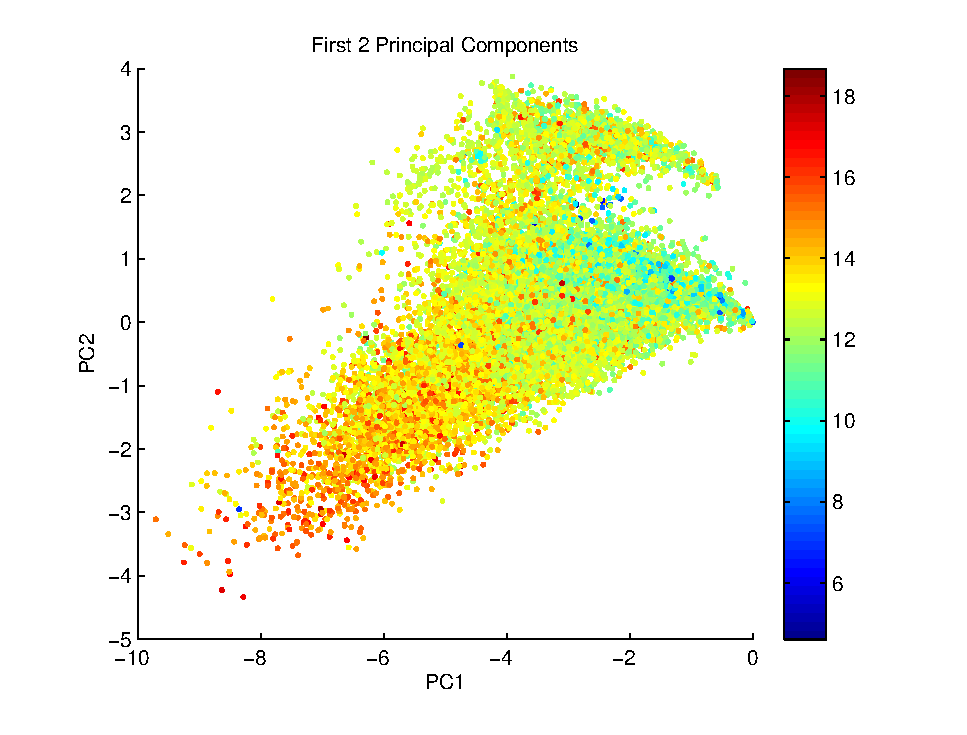
\includegraphics[scale=0.5]{First2PCs.eps}
 \caption{The first two pricipal components. The color represents the price (shown by the colorbar on the side)}
\end{figure}

While running a regression using the principal components works well, it is slightly better to run a regression using the 500 PCs along with the 7 city indicator variables. In effect, because the city is so much more important than the word data, we want to ensure that the regression has full access to the city data. Making this change improves the RMSE from 0.86 to 0.81.

\begin{figure}[H]
 \centering
 \begin{minipage}{.5\textwidth}
    \centering
    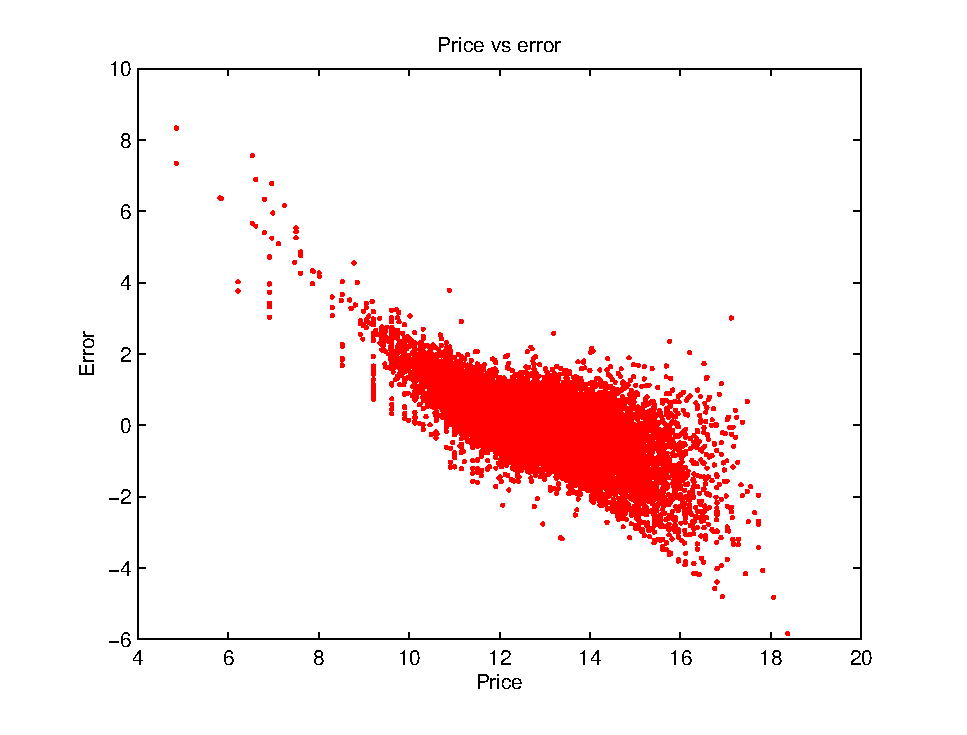
\includegraphics[width=6.0cm]{PCRPriceVsError.eps}
    \label{fig:fig1}
  \end{minipage}%
  \begin{minipage}{.5\textwidth}
    \centering
    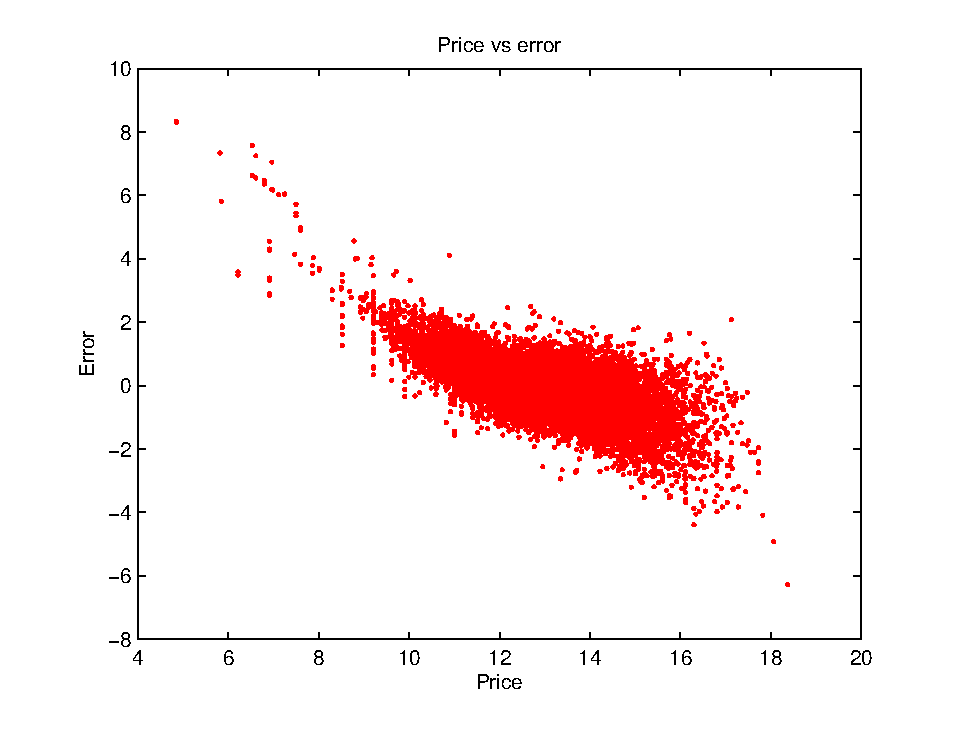
\includegraphics[width=6.0cm]{PCRPriceVsErrorWithCities.eps}
    \label{fig:fig2}
  \end{minipage}
 \caption{The errors of the PCR without cities (left) and with cities (right).
	  With the cities the curves on the edges are less pronounced}
\end{figure}

\section{Linear Regression with $L_1$ Regularization and Hand Crafted Features}
\subsection*{Simple Linear regression}
We also tried adding additional features to principal component feature space. We added feature interactions for the first 21 most-useful prinicpal components (i.e. we took their product to add $21^2$ new features). This gave a RMSE of 0.78. We also tried adding in a subset of the words (around 300 of them), feature selected using LASSO on the words and finding the highest weighted words. We also did this with the bigrams (adding less of them, about 200). Adding all of these features improved the error to 0.76. Note that these improvements only happened after choosing the optimal lambda (which varied depending on the number of features intuitively). 


\section{SVM to separate data}
\subsubsection*{Discriminative Method}
We noticed that while our model was good at predicting average-priced houses, it wasn't doing well at predicting very cheap houses. We attempted to solve this problem using an SVM.

We began with 500 principal components. We trained an SVM using MATLAB's built-in svm classifier on these PCs to identify cheap houses (houses in the 10th percentile or lower of all house prices). We then trained lasso regressions on both the cheap houses and the not-cheap houses. To classify a new point, we use the SVM to predict whether to house was cheap or expensive, then used the appropriate model. This gave a RMSE of 0.77. Unfortunately, the SVM is memory intensive and did not fit in the 50MB space limit.

\section{Kernel Regression}
\subsubsection*{Instance Based Method}
We also ran Kernel regression with a gaussian kernel. Storing the entire kernel matrix in memory is not possible, so we used several tricks to reduce memory usage. First, we used \emph{KMBOX} as a starting point and wrote memory-efficient code that tried to create the kernel matrix in segments instead of all at once. Second, instead of training on the full data set, we trained in a large fraction (11000 points) of the principal components.

We managed to get a RMSE of 0.73 using kernel regression, our best result and beating the second baseline. It's also likely that using the full data set would have given even better results. However, the method took to long to use as our final method (predicting 20000 points one-at-a-time took approximately 30 minutes). Thus, we looked into finding ways to run kernel regressions using less data.

\section{K-Means as centers of Radial Basis Functions for Kernel Regression}
\subsubsection*{Generative Method/Instance Based Method}
We first ran K-means to get 2000 mean-center points, then ran a kernel regression using these 2000 points. This gave a RMSE of 0.95. The means are not representative of the data as a whole.

When looking at the range of clusters, we saw that many clusters were nearly empty and mana clusters had 200+ points. The problem is that there are places where many houses are close together in the dimensionally-reduced feature space (and so are put into the same cluster), but their prices are very different. This is why using kernel regression on the whole dataset works much better: it can account for these bad spots, whereas the means alone cannot.

\begin{figure}[H]
 \centering
 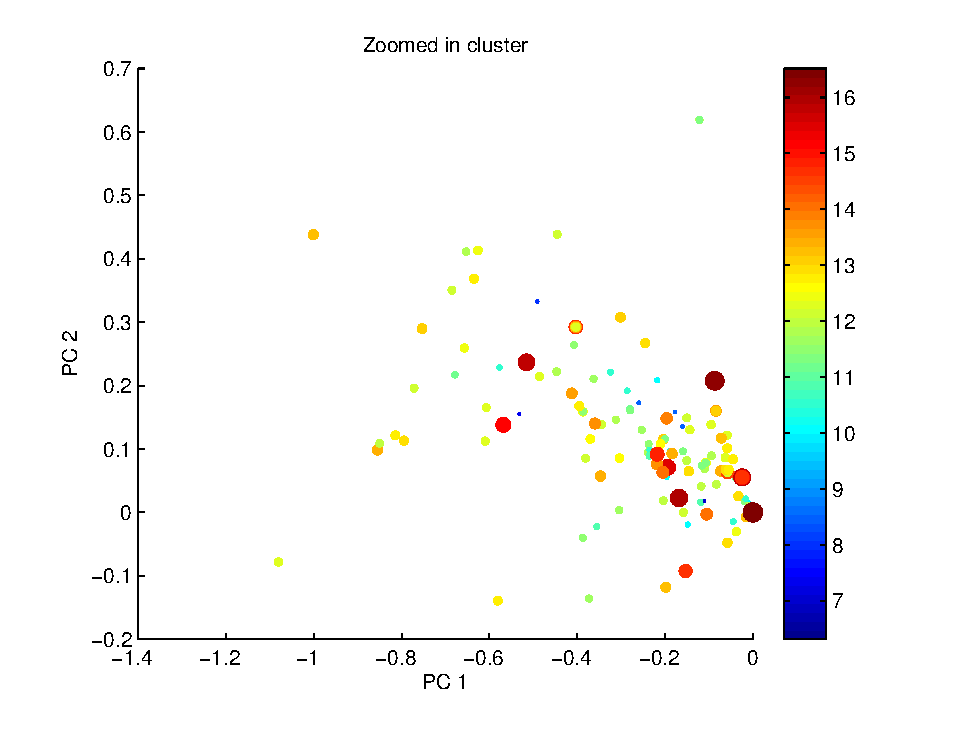
\includegraphics[scale=0.5]{ZoomedInCluster.eps}
 \caption{One of the larger clusters in our kmeans, zoomed in. Color and size show the price value of each point. As you can see, there are a large range of them all in very
	  close proximity, so using the mean of this cluster is not very informative.}
\end{figure}

\section{K-Means Clustering with Kernel Regression}
\subsubsection*{Generative Method/Instance Based Method}
An alternate attempt to reduce the size of the kernel method also involved k-means. We first clustered the data into 10 clusters, then ran a seperate kernel regression on each cluster. This ended up being terrible, with a RMSE of 1.22. Every cluster had about 2000 points in it, which is not a lot of data. Furthermore, whereas the 2000 mean-points are at least somewhat indicitive of the 'average data point', the 2000 points in a given cluster may be very distinct.

\section{Linear Regression with $L_1$ Regularization (LASSO)}
\subsection*{Simple Linear regression}
The last method we tried was a lasso regression using the full 5007 features. This performs quite well, giving a RMSE of 0.75. Using the full feature set gives more information and, with the right regularization, can perform better than using the dimensionallity reduced data. We used the matlab package \emph{glmnet} to quickly run the regression.

\section{Ensemble}
\subsubsection*{Putting it all together}
The final submission we used was an ensemble method which ended up being the best. We trained on about 75 percent of the data chose the weights with the rest of the data then used those weightings of the different methods on the testing set. We get 0.75 RMSE which is our best method yet. We might have been able to play around with how we split the data to get better results, but we thought that this split was fairly good.

The results can be summarized in the table below
\begin{center}
\begin{tabular}{|c | c|}
\hline
 Technique & RMSE \\ \hline
Lasso with 500 PCs from word/bigram & 0.86457 \\ \hline
Lasso with 500 PCs plus city data & 0.8135 \\ \hline
Lasso with hand-crafted features & 0.7632 \\ \hline
Lasso with SVM to identify cheap houses & 0.7754 \\ \hline
Kernel with 11000 points & 0.7352 \\ \hline
Kernel with 2000 mean points & 0.94641 \\ \hline
Clustering with Kmeans and Kernel Regression & 1.2169\\ \hline
Lasso with all 5007 features & 0.75695 \\ \hline
Ensemble & 0.7545 \\ \hline
\end{tabular}
\end{center}

\section{Conclusion}
The best method we found was kernel regression using a gaussian kernel, which worked well but had issues with time and memory. Although we tried multiple fancy techniques with dimensionality reduction, a straight lasso regression with all of the data preformed very very well.


\end{document}
